\documentclass[a4paper,12pt]{article}
\usepackage[verbose,a4paper,tmargin=2cm,bmargin=3cm,lmargin=2cm,rmargin=2cm]{geometry}
\usepackage[utf8]{inputenc}
\usepackage{polski}
\usepackage[latin2]{inputenc}
\usepackage{caption}
\usepackage{graphicx}
\usepackage[polish]{babel}
\usepackage{color}
\title{Kompo - sprawko}
\author{Patryk Lisik}
\date{June 2018}
\definecolor{dkgreen}{rgb}{0,0.6,0}
\definecolor{ltgray}{rgb}{0.5,0.5,0.5}

\usepackage{listings}
\lstset{%
  	backgroundcolor=\color{white},
  	basicstyle=\footnotesize,
  	breakatwhitespace=false,
  	breaklines=true,
  	captionpos=b,
  	commentstyle=\color{dkgreen},
  	deletekeywords={...},
  	escapeinside={\%*}{*)},
  	extendedchars=true,
  	frame=single,
  	keepspaces=true,
  	keywordstyle=\color{blue},
  	language=SQL,
  	morekeywords={*,modify,MODIFY,...},
  	numbers=left,
  	numbersep=15pt,
  	numberstyle=\tiny,
  	rulecolor=\color{ltgray},
  	showspaces=false,
  	showstringspaces=false, 
  	showtabs=false,
  	stepnumber=1,
  	tabsize=4,
  	title=\lstname
}
\begin{document}

\begin{titlepage}
\vspace{10cm}


\centering
{\center\huge\ Programowanie komponentowe \par}
\vspace{1.5cm}
{\center\huge\bfseries Sprawozdanie z pracy projektowej  \par}
\vspace{1.5cm}
{\center\huge\bfseries Kalendarz}

\vspace{6cm}


\begin{flushright}
\begin{tabular}{lll}
Patryk & Lisik & 210254 \\ 
Dominika & Wójcik  & 210355 \\ 
\end{tabular} 
\end{flushright}

\vspace{5cm}

\begin{center}
\textbf{Infromatyka, sem IV \\}
\textbf{2017/2018}
\end{center}
 

\end{titlepage}

Stworzona aplikacja jest kalendarzem przechowującym, wydarzenia, kontakty oraz powiadomienia. Pozwala utrwalać oraz pobierać dane za pomocą formatu XML, serializacji binarnej Javy oraz bazy danych MySQL. Użytkownikowi zostaje udostępniony interfejs graficzny zaprezentowany w podpunktach 3.2.1 -  3.2.3. 
       
\section{Najważniejsze klasy warstwy danych projektu}
Warstwa danych umożliwia przechowywanie danych o osobach wydarzeniach i powiadomieniach. Osoby są reprezentowane przez klasę Person posiadające dwa pola imię i nazwisko będące stringami. Wydarzenie jest reprezentowane poprzez klasę Event, na którą składają się opis, data początku, końca oraz lista powiadomień. Powiadomienie jest reprezentowane przez klasę Notafication, na którą składają się opis powiadomienia oraz jego data. 
Warstwa danych przechowuje wyżej wymienione obiekty.

Stworzono dwie implementacje warstwy danych bez połączenia, oraz z połączaniem do bazy danych. Druga z nich rozszerza pierwszą dodając metody pozwalające zapisać zmiany do bazy danych lub wczytać stan z bazy. Połączanie z bazą danych zostało zaimplementowane na zasadzie migawki. Gdy tworzona jest nowa instancja klasy wczytywane są dane z bazy. W tracie wykonania programu w buforze zapisywane są kwerendy zmieniające stan bazy do tożsamego z tym zapisanym w pamięci. 

\begin{minipage}{\textwidth}

    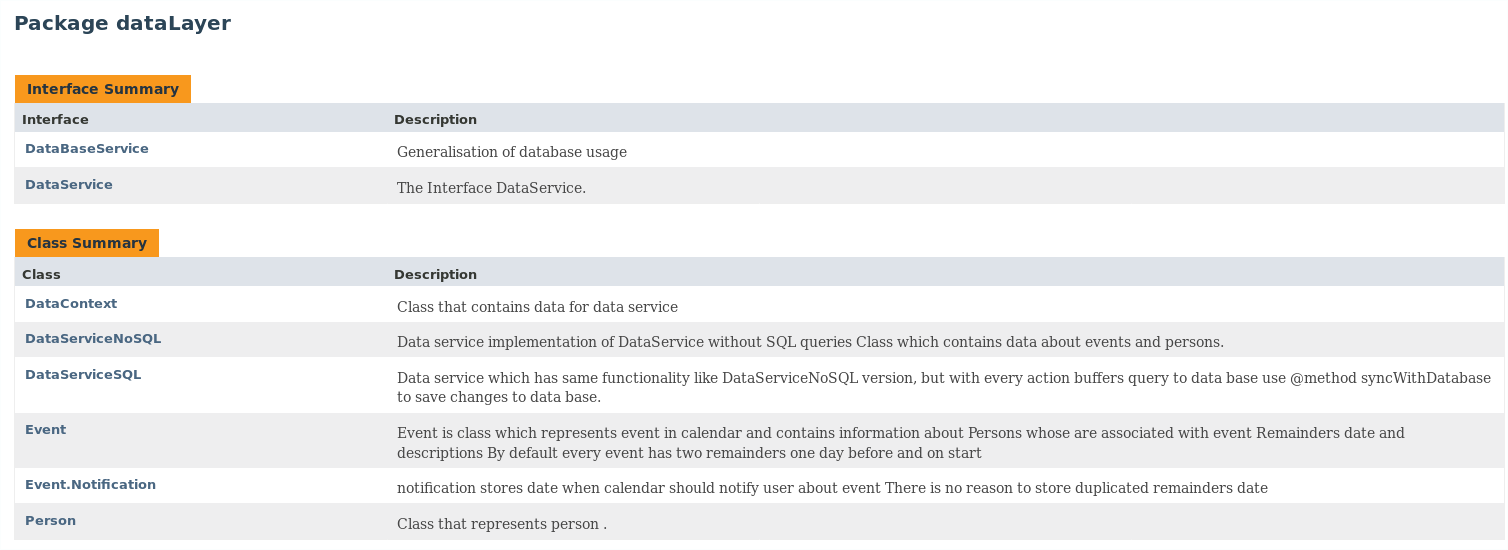
\includegraphics[width=\textwidth]{./screen/dataLayer/PackageDataLayer.png}
        \captionof{figure}{Dokumentacja package'u dataLayer}
    \label{dataLayer_pkg}

\end{minipage}

\begin{minipage}{\textwidth}

    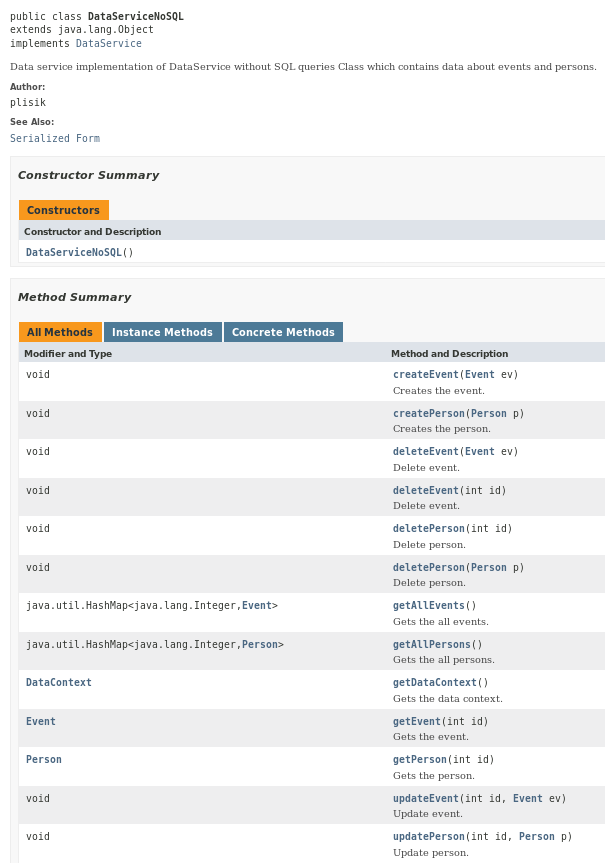
\includegraphics[width=\textwidth]{./screen/dataLayer/DataServiceNoSQL.png}
        \captionof{figure}{Dokumentacja klasy DataServiceNoSQL}
    \label{DataServiceNoSQL}

\end{minipage}

\begin{minipage}{\textwidth}

    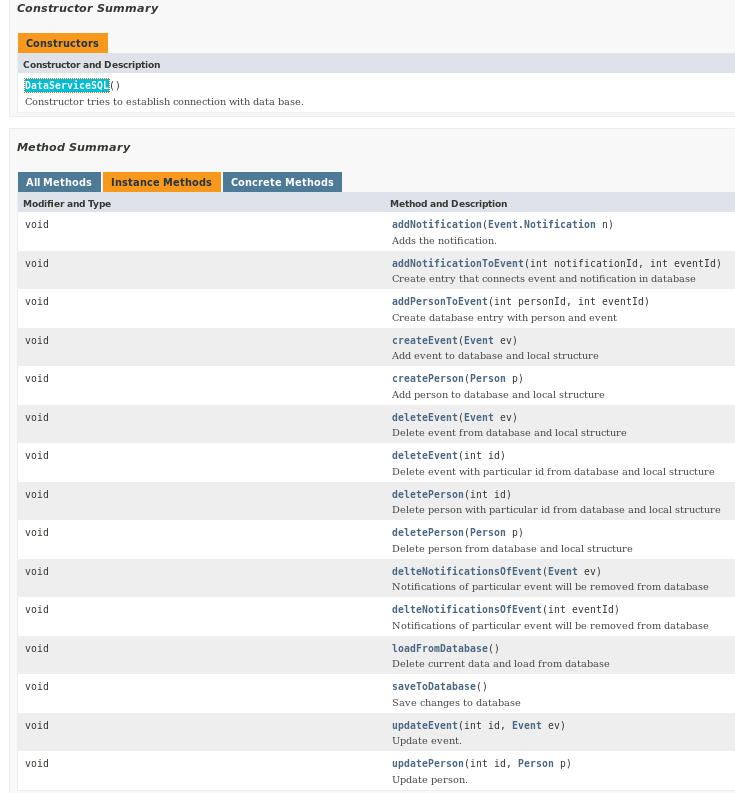
\includegraphics[width=\textwidth]{./screen/dataLayer/DataServiceSQL.png}
        \captionof{figure}{Dokumentacja klasy DataServiceSQL}
    \label{DataServiceSQL}

\end{minipage}

\begin{minipage}{\textwidth}

    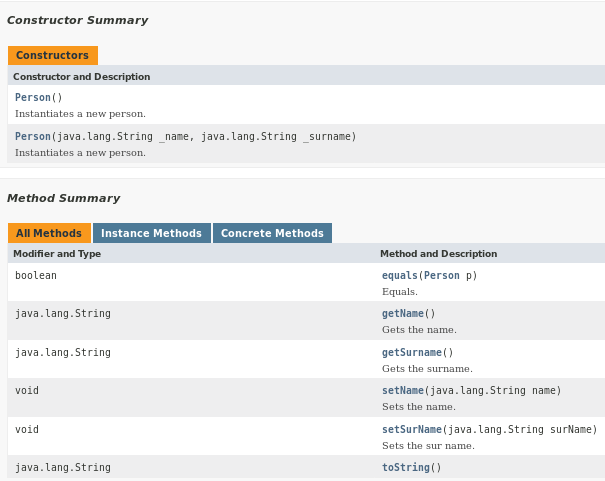
\includegraphics[width=\textwidth]{./screen/dataLayer/Person.png}
        \captionof{figure}{Dokumentacja klasy Person}
    \label{Person}

\end{minipage}

\begin{minipage}{\textwidth}

    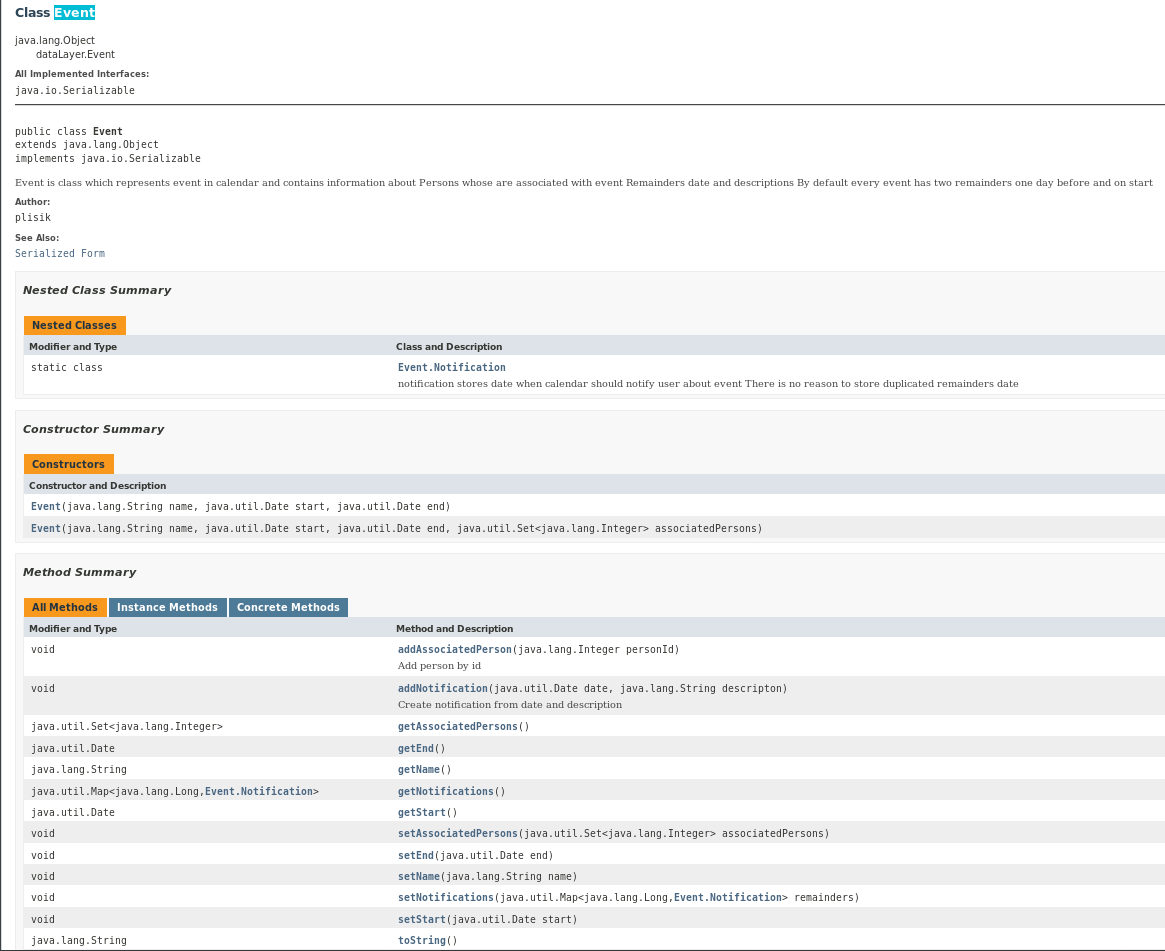
\includegraphics[width=\textwidth]{./screen/dataLayer/Event.png}
        \captionof{figure}{Dokumentacja klasy Event}
    \label{Event}

\end{minipage}


\section{Najważniejsze klasy warstwy logiki}
       Warstwa logiki umożliwia manipulowanie warstwą danych. Poza tworzeniem obiektów warstwy danych warstwa logiki umożliwia:
\begin{enumerate}
 \item znalezienie wydarzeń między datami
 \item znalezienie wydarzeń w danym dniu
 \item posortowanie wydarzeń po dacie 
 \item posortowanie wydarzeń po ilości uczestniczących osób
 \item zapis i odczyt z XML i serializacji binarnej
 \item zapis do formatu odt(OpenOffice)
 \item informowanie o zmianie stanu kolekcji
\end{enumerate}

Do seralizowania danych do formatu XML wykorzystano bibliotekę XStream.

Zapis i odczyt z formatów standardowych zrealizowano za pomocą wzorca projektowego strategi. Stworzone zostały interface'y Importer i Saver które uogólniają zapis i odczyt z dowolnego formatu. Na ich podstawie powstały konkretne klasy jak XMLSaver,XMLImporter,ODTSaver itd.


Zaimplementowane zostało automatyczne uruchamianie powiadomień. Odpowiada za to klasa EventNotifiactionPublisher posiadająca dwa wewnętrzne interfac'y:
\begin{itemize}
\item NotificationReciver -- uogólniający dowolnego odbiorcę powiadomień, do którego o odpowiednim czasie(zdefiniowanym przez samo powiadomienie) zostanie wysłana teść powiadomienia(poprzez wywołanie odpowiedniej metody).
\item NotifiactionSource -- uogólnienie źródła powiadomień. oczekuje się że wywołana odpowiednią metodę jeśli lista powiadomień zostanie zmieniona. 
\end{itemize}

Sama czynność wywoływania metody w odpowiednim czasie została zrealizowana za pomocą kalsy TimerTask. 


   

\begin{minipage}{\textwidth}

    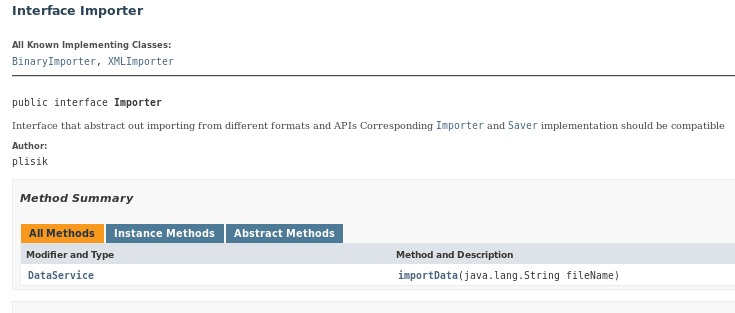
\includegraphics[width=\textwidth]{./screen/logicLayer/Importer.png}
        \captionof{figure}{Dokumentacja interfac'u Importer}
    \label{Importer}

\end{minipage}

\begin{minipage}{\textwidth}

    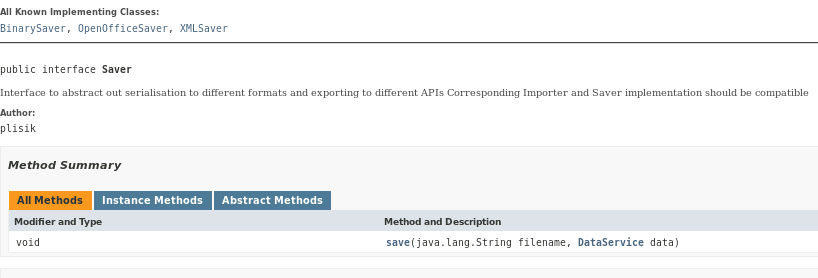
\includegraphics[width=\textwidth]{./screen/logicLayer/Saver.png}
        \captionof{figure}{Dokumentacja interfac'u Saver}
    \label{Saver}

\end{minipage}

\begin{minipage}{0.75\textwidth}

    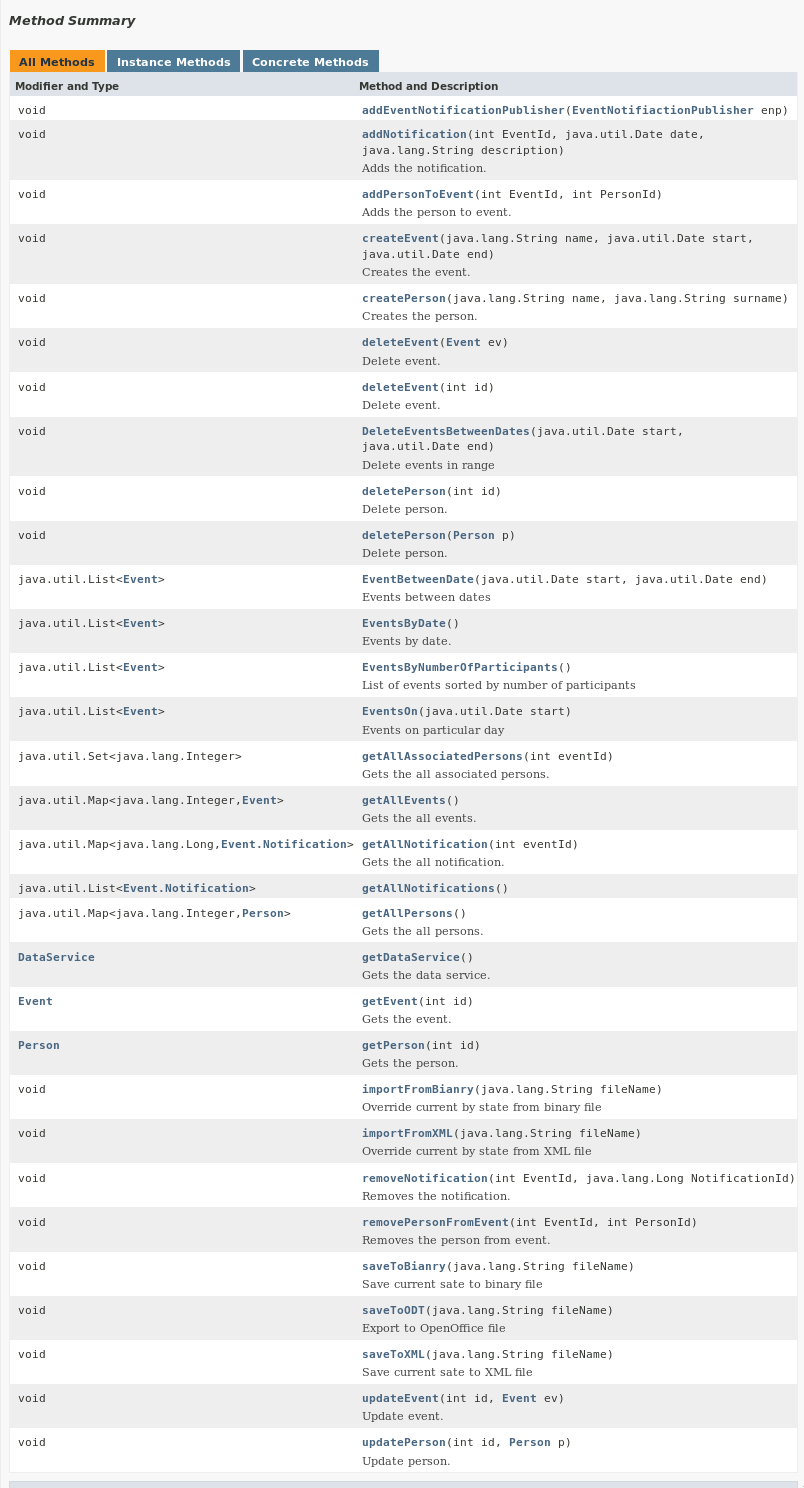
\includegraphics[width=\textwidth]{./screen/logicLayer/LogicLayerImpl.png}
        \captionof{figure}{Dokumentacja klasy LogicLayerImpl}
    \label{LogicLayerImpl}

\end{minipage}

\begin{minipage}{\textwidth}

    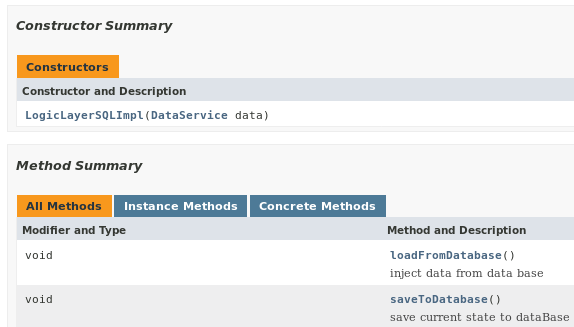
\includegraphics[width=\textwidth]{./screen/logicLayer/LogicLayerSQLImpl.png}
        \captionof{figure}{Dokumentacja klasy LogicLayerSQLImpl}
    \label{LogicLayerSQLImpl}

\end{minipage}

\begin{minipage}{\textwidth}

    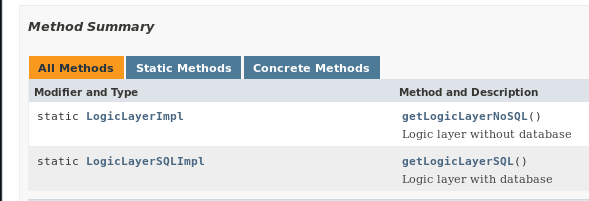
\includegraphics[width=\textwidth]{./screen/logicLayer/LogicLayerFactory.png}
        \captionof{figure}{Dokumentacja klasy LogicLayerFactory}
    \label{LogicLayerFactory}

\end{minipage}

\begin{minipage}{\textwidth}

    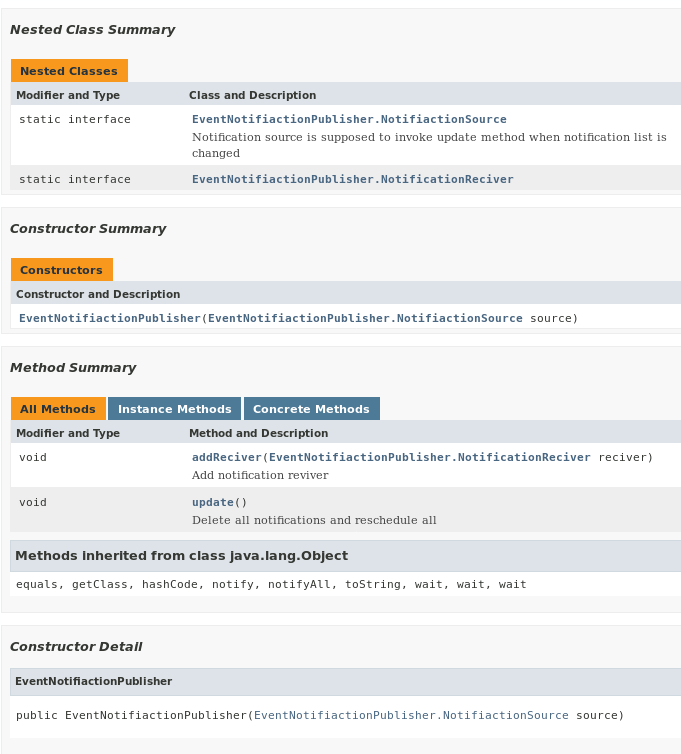
\includegraphics[width=\textwidth]{./screen/logicLayer/EventNotificationPublisher.png}
        \captionof{figure}{Dokumentacja klasy EventNotificationPublisher}
    \label{LogicLayerFactory}

\end{minipage}

\section{Warstwa interfejsu}
\subsection{Najważniejsze klasy warstwy interfejsu}
Główną klasą odpowiedzialną za uruchomienie wszystkich mechanizmów związanych z widokiem aplikacji jest klasa MainWindow.
Podczas uruchomienia aplikacji powstaje obiekt klasy Calendar odpowiedzialny za główny widok okna oraz utworzenie słuchaczy, czyli obiektów klasy implementującej interfejs ActionListener. Pozostałe klasy takie jak ContactsView, DayView, MonthView i inne implementują pozostałe elementy kalendarza.
W warstwie prezentacji znajduje się także klasa StateContainer odpowiedzialna za zarządzanie  generowanymi podczas działania programu zdarzeniami.

\begin{minipage}{.75\textwidth}

    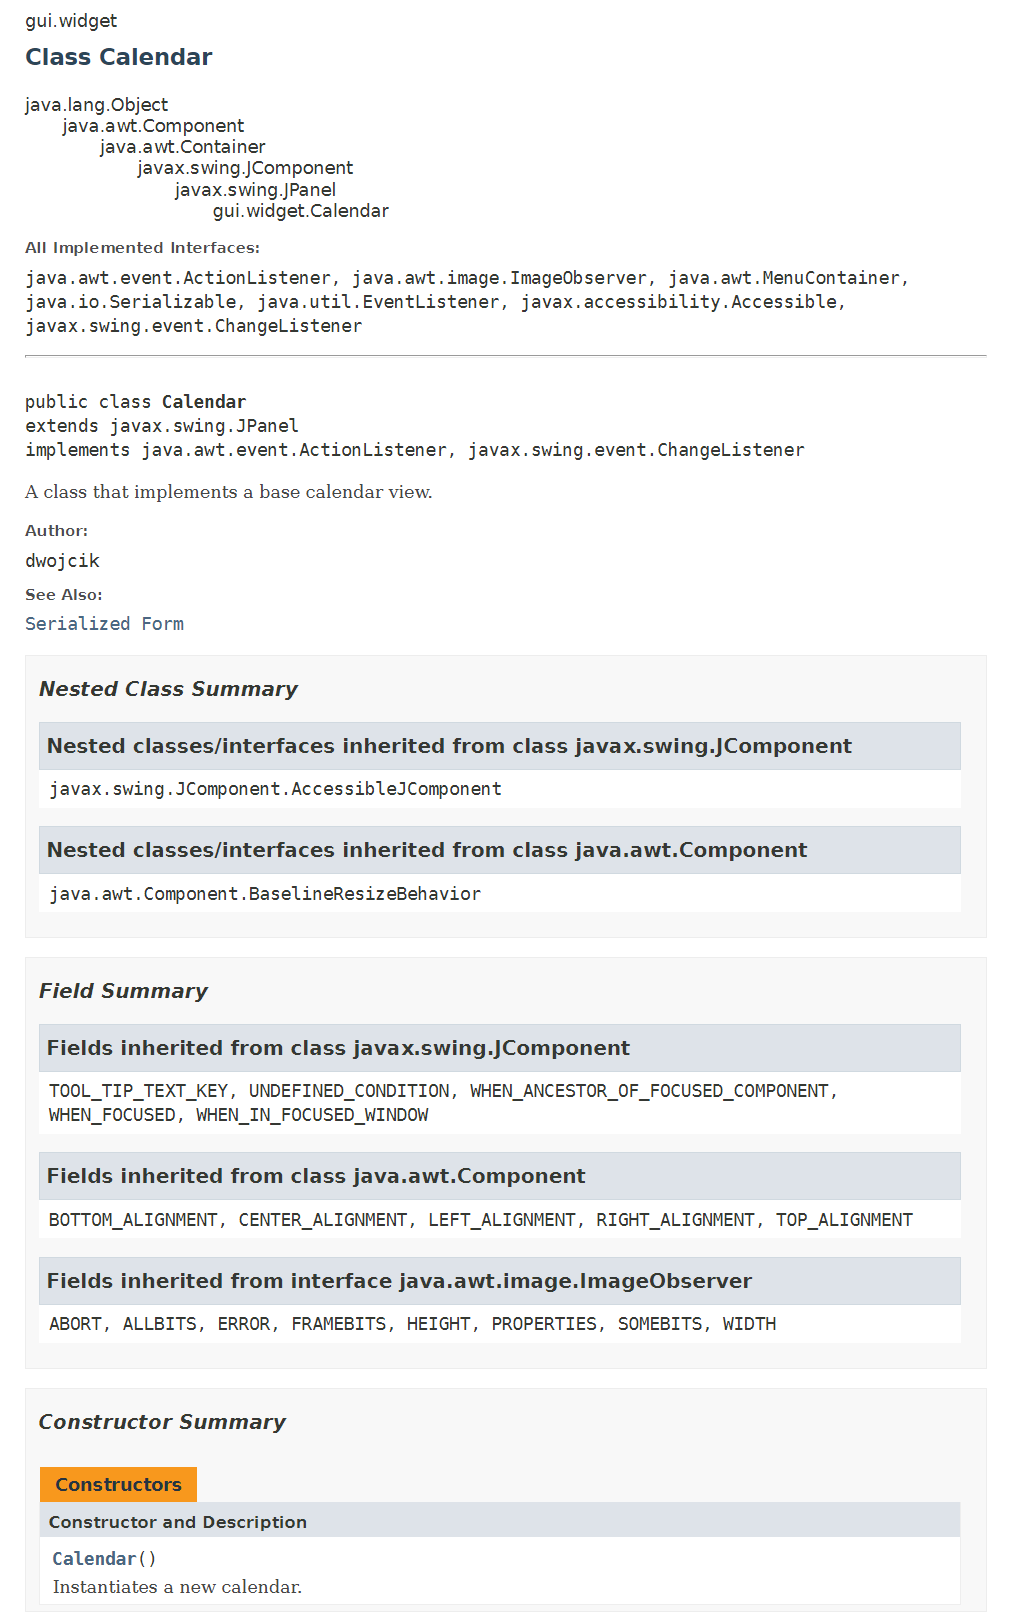
\includegraphics[width=\textwidth]{./screen/GUI/calendar.png}
        \captionof{figure}{Dokumentacja klasy calendar}
    \label{MainViewLinux}

\end{minipage}

\begin{minipage}{.75\textwidth}

    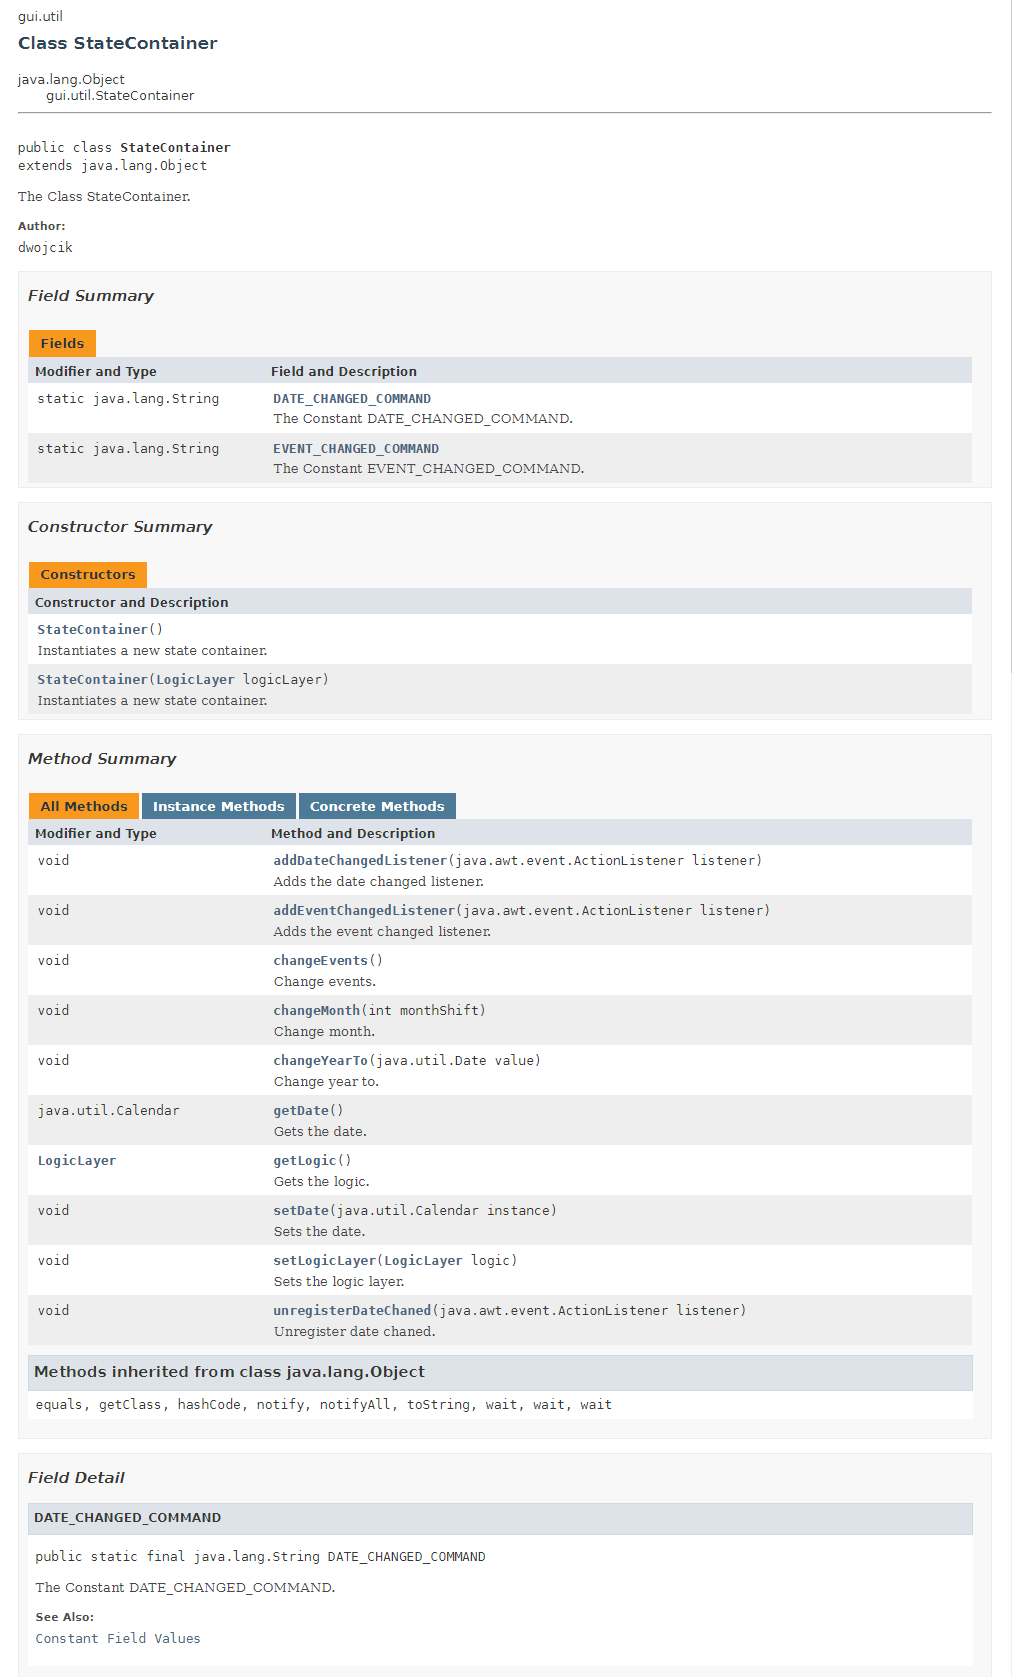
\includegraphics[width=\textwidth]{./screen/GUI/stateContainer.png}
        \captionof{figure}{Dokumentacja klasy stateContainer}
    \label{MainViewLinux}

\end{minipage}

\subsection{Zrzuty ekranu najważniejszych widoków działającej aplikacji}
\subsubsection{Główne okno kalendarza ''organizera''}

\begin{minipage}{\textwidth}

    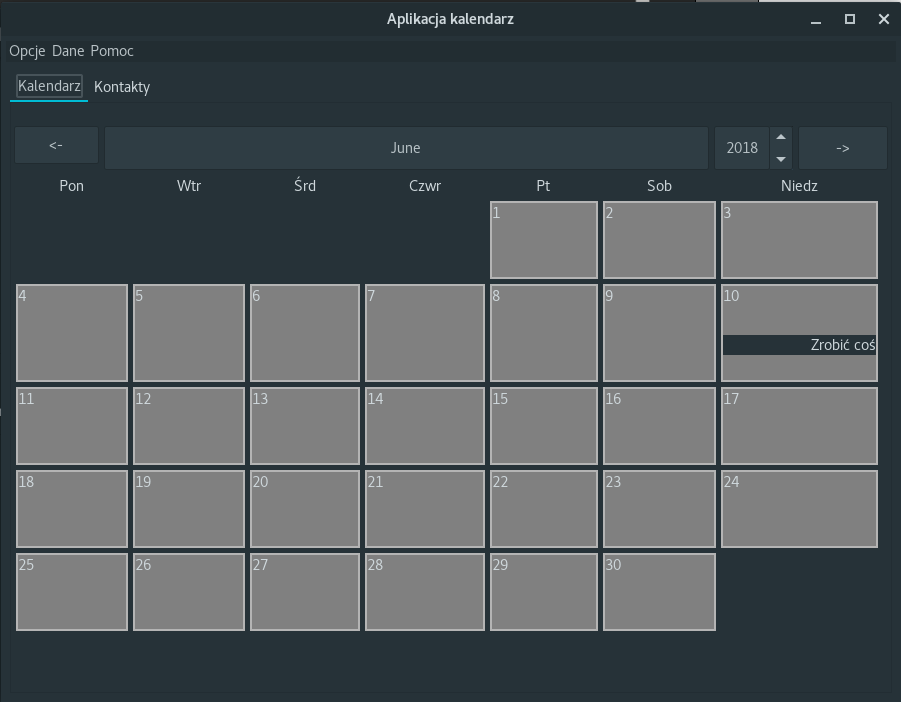
\includegraphics[width=\textwidth]{./screen/AppScreen/MainViewLinux.png}
        \captionof{figure}{Główne okono kalendarze w sytstemi linux}
    \label{MainViewLinux}

\end{minipage}

\subsubsection{Okienko ''O programie''}

\begin{center}
\begin{minipage}{0.5\textwidth}

    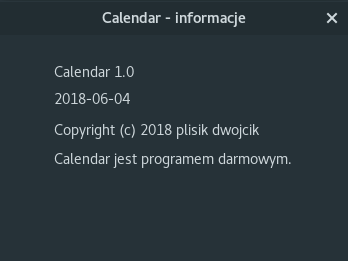
\includegraphics[width=\textwidth]{./screen/AppScreen/AboutDialog.png}
        \captionof{figure}{Okno pokazujące informacje o programie}
    \label{MainViewLinux}

\end{minipage}
\end{center}

\subsubsection{Okienka dialogowe zapisujące/odczytujące dane i ustawienia do/z bazy/pliku XML}
\begin{minipage}{0.5\textwidth}

    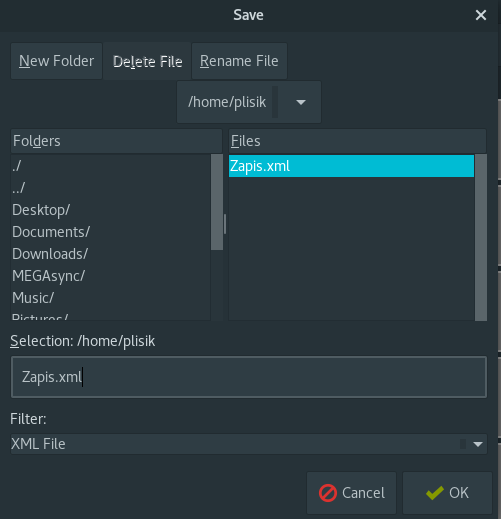
\includegraphics[width=\textwidth]{./screen/AppScreen/SaveTo.png}
        \captionof{figure}{Okno zapisu do XML}
    \label{MainViewLinux}

\end{minipage}
\begin{minipage}{0.5\textwidth}

    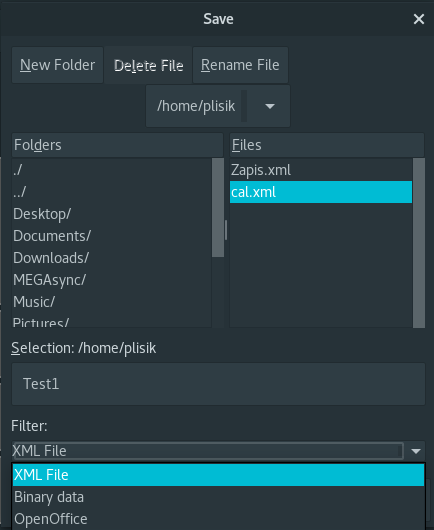
\includegraphics[width=\textwidth]{./screen/AppScreen/SaveToAll.png}
        \captionof{figure}{Wybór formatu zapisu w oknie zapisu}
    \label{MainViewLinux}

\end{minipage}

\subsection{Jasny i czytelny opis klawiszy funkcyjnych i przycisków obsługujących aplikację}
\section{Postać bazy danych z zapisanymi informacjami o zdarzeniach}
W projekcie zastosowano bazę danych MySQl w wersji 8.0.11. Wybór ten podyktowany był znacznie prostszą konfiguracją w systemie linux(wystarczy jedna komenda w terminalu).
\lstinputlisting[language=sql,caption={Skrypt tworzący bazę danych}]{../SQL_init.sql}


\begin{lstlisting}[style=DOS]
mysql> SELECT * FROM events;
+----+------+---------------------+---------------------+
| id | name | start               | end                 |
+----+------+---------------------+---------------------+
|  1 | test | 2018-06-13 22:00:00 | 2018-06-16 06:57:18 |
+----+------+---------------------+---------------------+
1 row in set (0.00 sec)

mysql> SELECT * FROM persons;
+----+--------+---------+
| id | name   | surname |
+----+--------+---------+
|  1 | patryk | lisik   |
+----+--------+---------+
1 row in set (0.00 sec)

mysql> SELECT * FROM notifications;
+----+------------------------------+---------------------+
| id | description                  | notify_date         |
+----+------------------------------+---------------------+
|  0 | is starting now              | 2018-06-13 22:00:00 |
|  1 | is going to start in one day | 2018-06-12 22:00:00 |
+----+------------------------------+---------------------+
2 rows in set (0.00 sec)

mysql> SELECT * FROM notifications_events;
+----------+-----------------+
| event_id | notification_id |
+----------+-----------------+
|        0 |               1 |
|        1 |               1 |
+----------+-----------------+
2 rows in set (0.00 sec)
\end{lstlisting}
\captionof{lstlisting}{Listing z stanu bazy danych po wykonaniu kilku operacji}
\section{Podsumowanie i ewentualne uwagi grupy nt. projektu. }

Programistyczna strona projektu, poza kilkoma nieporozumieniami związanymi z wykorzystaniem klas zaimplementowanych przez drugą osobę, nie sprawiła większych problemów. Popełniliśmy natomiast kilka błędów związanych z używanymi narzędziami:
\begin{itemize}
\item Zbyt późno zaczęliśmy używać Mavan'a do zarządzania zależnościami, przez co często traciliśmy czas na doinstalowywanie bibliotek i edycję pliku "BuildPatch".

\item Brak tworzenia testów automatycznych i ciągłej integracji poskutkował kilkoma regresami i trudnymi do zlokalizowania błędami wynikającymi z niewielkich zmian. 
\end{itemize}

\end{document}
